\documentclass[11pt,a4paper,titlepage, ngerman]{article}

\usepackage[utf8]{inputenc}	% Diese Pakete sind
\usepackage[T1]{fontenc}		% für die Verwendung 
\usepackage{ngerman}			% von Umlauten im tex-file
\usepackage{lmodern}			% Schriftart, die am Bildschirm besser lesbar ist
\usepackage{graphicx}			% Zum Einbinden von Formeln
\usepackage{url}					% Zur Darstellung von Webadressen
\usepackage{siunitx}
\usepackage{amsmath}			% für equation*
\usepackage{subcaption}
\usepackage{wrapfig}

\begin{document}
%	\setlength{\parindent}{0em} 
	
	\begin{titlepage}
		\centering
		{\scshape\LARGE Versuchsbericht zu \par}
		\vspace{1cm}
		{\scshape\huge S2 -- Experimentieren, und dann?\par}
		\vspace{2.5cm}
		{\LARGE Gruppe 10 Mi\par}
		\vspace{0.5cm}
		{\large Alex Oster (E-Mail: a\_oste16@uni--muenster.de) \par}
		{\large Jonathan Sigrist (E-Mail: j\_sigr01@uni--muenster.de) \par}
		\vfill
		durchgeführt am 25.10.2017\par
		betreut von\par
		{\large Dr. Anke \textsc{Schmidt}}
		
		\vfill
		
		{\large \today\par}
	\end{titlepage}
		
	\tableofcontents
	
	\newpage
	
	\section{Einleitung}
		\label{Einleitung}
		
		
		\glqq Die Gravitationskonstante $g$ besitzt in der Stadt Münster einen Wert von \SIrange{10,5}{11}{m/s^2}.\grqq
		
		Zu dieser Aussage führten die Ergebnisse einer Fallgeschwindigkeitsmessung an der WWU.
		Hierbei wurden die Geschwindigkeiten einer fallenden Metallkugel an zwei verschiedenen Punkten, mit Hilfe von Lichtschranken gemessen. Dadurch ließ sich die Fallbeschleunigung und damit die Gravitationskonstante bestimmen.
		
		Dieser neu gemessene Wert steht in Konflikt mit dem aktuellen Wert der PTB von $g = \SI{9.813}{\meter\per\second\squared}$ und es steht nun zur Diskussion, ob die PTB ihren derzeitigen Wert ändern muss.
		
		In diesem Bericht beschäftigen wir uns damit, diese Aussage zu widerlegen.
		Dazu messen wir die Zeit von Pendelschwingungen und berechnen aus Fadenlänge und gemessener Zeit die Gravitationskonstante. Um ein möglichst genaues Ergebnis zu erhalten, führen wir mehrere Messungen mit verschiedenen Fadenlängen durch.
		
	\section{Methoden}
		
		\subsection{Mathematisches Pendel}
		\label{pendel}
		
		Wir betrachten für die Auswertung unserer Messungen das Modell des mathematischen Pendels unter folgenden Annahmen:
		\begin{enumerate}
			\item Die gesamte Masse $m$ ist im Schwerpunkt vereinigt (Massepunkt).
			\item Der Massepunkt $m$ ist durch einen masselosen Faden (starre Verbindung) der Länge $L$ mit dem Aufhängepunkt verbunden.
			\item Die Bewegung erfolgt ohne Reibung.
			\item Das Pendel wird nur leicht ausgelenkt ($\sin \varphi \approx \varphi$).
		\end{enumerate}
		In Abb. \ref{fig:matpendel} ist dies schematisch dargestellt. $\vec{G}$ sei die Gewichtskraft.
		Zu beachten ist, dass $\varphi$ deutlich kleiner ist, als in der Abbildung dargestellt.
		
		\begin{figure}[ht]
			\centering
			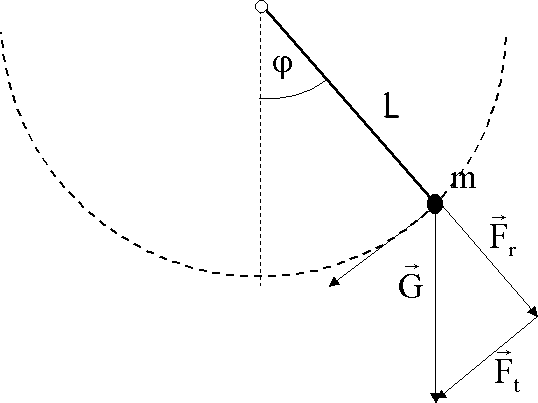
\includegraphics[scale=0.4]{mathematischesPendel.png}		
			\caption{mathematisches Pendel}
			\label{fig:matpendel}
		\end{figure}
		
		Die Differenzialgleichung des frei schwingenden Pendels
		\begin{equation*}
		\ddot{\varphi}+\left( \frac{g}{L}\right)  \sin \varphi = 0
		\end{equation*}
		lässt sich unter den Annahmen lösen, mit 
		\begin{equation}
		\label{eq:g}
		\omega =  \sqrt{\frac{g}{L}}, \quad 
		T =  2\pi \sqrt{\frac{L}{g}}, \quad
		g = \left(\frac{2 \pi}{T}\right)^2 L.
		\end{equation}
		
%		\begin{figure}[ht]
%			\centering
%			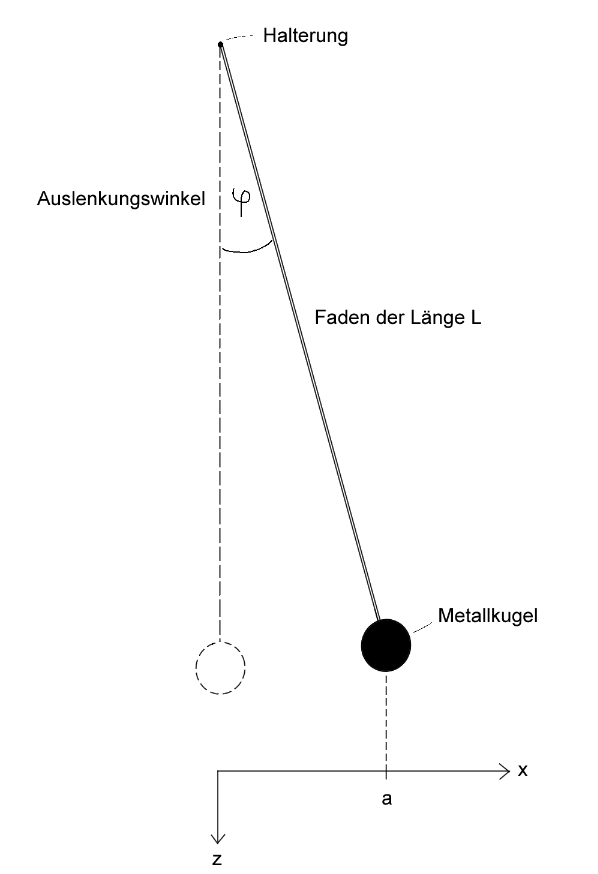
\includegraphics[width=\textwidth]{Pendel.png}		
%			\caption{Versuchsskizze}
%			\label{fig:pendel}
%		\end{figure}
		
		Wie in Abb. \ref{fig:matpendel} dargestellt, wurde die Kugel unter einer kleinen Auslenkung $\varphi_0$ losgelassen.
		Wir haben die Zeit gemessen, welche die Metallkugel benötigt hat, um eine bestimmte Anzahl Schwingung zu durchlaufen, also bis die Metallkugel wieder ca. bei $\varphi = \varphi_0$ angekommen ist.
		Das war gerade dann der Fall wenn die Kugel ihre Bewegungsrichtung gewechselt hat und somit leicht abzuschätzen.
		Wir haben jeweils mehrere Schwingungen in einer Messung zusammengefasst, um die Ungenauigkeiten von der Zeitmessung möglichst klein zu halten. 
		
		Die Zeit wurde mit einer handelsüblichen digitalen Stoppuhr gemessen, welche zwei Nachkommastellen anzeigt.
		Eine Ungenauigkeit der Uhr ist uns nicht bekannt.
		Zum Messen der Seillänge haben wir ein Maßband von zwei Metern Länge benutzt. Die Millimeter-angaben konnten leicht abgelesen werden.
		Auch hier ist uns eine Ungenauigkeit des Maßstabes nicht bekannt.
		Der Durchmesser von der Kugel betrug \SI{3}{\centi\meter} und wird als absolut angesehen.
		
		Für zwei Fadenlängen wurden viele Schwingungen gemessen und für vier weitere weniger.
		Dadurch konnten zusätzliche Referenzwerte geliefert werden, welche ebenfalls gegen die Behauptung gehen.
		
	\section{Messung}
	\label{Messung}
		Die Unsicherheiten in Tab. \ref{tab:unsicherheiten} sind gegeben durch
		$u_\text{Uhr} = \frac{\SI{0,01}{\second}}{2\sqrt{3}}\approx \SI{2,89}{\milli\second}$ und $u_\text{Reaktion} = \frac{\SI{0,1}{\second}}{2\sqrt{6}} \approx \SI{20,4}{\milli\second}$.
		Daraus folgt die kombinierte Unsicherheit $u_\text{Zeit} = \sqrt{\left( u_\text{Uhr}\right) ^2+\left( u_\text{Reaktion}\right) ^2}\cdot\frac{1}{n} \approx \frac{\SI{20,6}{\milli\second}}{n}$ pro Schwingung ($n$ sei die Anzahl an Perioden pro Messung).\\
		Die Unsicherheit zur Länge durch $u_\text{Länge} = \frac{\SI{0,001}{\meter}}{2\sqrt{6}} \approx \SI{0,204}{\milli\meter}$.
			
		\begin{table}[ht]
			\centering
			\begin{tabular}{S|S|S||S}
				\hline
				{Digitale Stoppuhr} & {Reaktionszeit} & {Zeitlich} & {Maßband}\\
				\hline
				\SI{2,887}{\milli\second} & \SI{20,41}{\milli\second} & \SI{20,616}{\milli\second\per{n}} & \SI{0,2041}{\milli\meter} \\
				\hline
			\end{tabular}
			\caption{Unsicherheiten der Messinstrumente}
			\label{tab:unsicherheiten}
		\end{table}
			
		Es folgen die durchschnittlichen Zeiten für die Periodendauern, welche sich durch die durchgeführten Messungen für verschiedene Fadenlängen $L$ ergaben.
		\vspace{0.25cm} 
		
		\begin{description}
			
			\item[Fadenlänge 1:]($L_1 = \SI{111,6 +- 0,02}{cm}$)\\
			Für die erste Fadenlänge haben wir 110 Schwingungsdauern in 10er Schritten gemessen (D.h. jeweils die Periodendauer für zehn Schwingungen auf einmal). \\
			Die durchschnittliche Zeit für eine Pendelschwingung betrug hierbei: \SI{2.134 +- 0,002}{s}.
			
			\item[Fadenlänge 2:]($L_2 = \SI{104,5 +- 0,02}{cm}$)\\ 				 
			Bei dieser und der folgenden Messung haben wir nur 20 Perioden in 5er Schritten gemessen. Hier betrug die durchschnittliche Zeit für eine Pendelschwingung: \SI{2,060 +- 0,004}{s}.
			
			\item[Fadenlänge 3:]($L_3 = \SI{86,9 +- 0,02}{cm}$)\\ 			
			Es wurden nur 20 Schwingungen in 5er Schritten betrachtet. Dabei ergab sich für eine Pendelschwingung die durchschnittliche Zeit: \SI{1,879 +- 0,004}{s}.	
			
			\item[Fadenlänge 4:]($L_4 = \SI{65,8 +- 0,02}{cm}$)\\ 				
			Diese Messung und die Folgende betrachten wir 25 Perioden, ebenfalls in 5er Schritten. Die durchschnittliche Zeit für eine Pendelschwingung betrug hierbei: \SI{1,636 +- 0,004}{s}.
			
			\item[Fadenlänge 5:]($L_5 = \SI{116,3 +- 0,02}{cm}$)\\ 				
			Es wurden 25 Schwingungen in 5er Schritten betrachtet. Hier erhalten wir für eine Pendelschwingung die durchschnittliche Zeit: \SI{2,174 +- 0,004}{s}.
			
			\item[Fadenlänge 6:]($L_6 = \SI{92,6 +- 0,02}{cm}$)\\ 				
			Da wir bei den letzten vier Messungen nicht viele Schwingungen betrachtet haben, haben wir für die sechste Fadenlänge noch einmal 100 Schwingungsdauern gemessen. Dabei haben wir eine Länge $L$ gewählt, die circa \SI{20}{cm} von der ersten abwich, um mehrere Werte für \glqq deutlich\grqq{} unterschiedliche Längen $L$ zu erhalten. 
			Hierbei betrug die durchschnittliche Zeit für eine Pendelschwingung \SI{1,936 +- 0,002}{s}.
				
		\end{description}
		
	\section{Datenanalyse}
		\label{Auswertung}	
	
		In Tab. \ref{tab:werteTabelle} sieht man die Ergebnisse der Analyse.
		Diese Werte stimmen in etwa mit den Werten aus dem Vortrag\footnote{gemeint ist der Vortrag von Frau Dr. Anke Schmidt vom 25.10.} überein.
		\begin{table}[ht]
			\centering
			\begin{tabular}{l|S|S|S}
				\hline
				& {Messung 1} & {Messung 2} & {Mehrfachmessung} \\
				\hline
				$g$ & \SI{9,807 +- 0,190}{\meter\per\second\squared}
				& \SI{9,907 +- 0,021}{\meter\per\second\squared}
				& \SI{9,643 +- 0,111}{\meter\per\second\squared}\\
				\hline
			\end{tabular}
			\caption{Ergebnisse der Messungen}
			\label{tab:werteTabelle}
		\end{table}
		
		Die Ergebnisse 1 und 2 aus Tab. \ref{tab:werteTabelle} folgen direkt nach der Gl. (\ref{eq:g}).
		Dabei sind die Messunsicherheiten gegeben durch
		\begin{equation*}
			u(g) = \sqrt{
				\left( \frac{\partial f}{\partial T} u(T) \right)^2 +
				\left( \frac{\partial f}{\partial L} u(L) \right)^2
			}
			= g \sqrt{\left(\frac{u(L)}{L}\right)^2 + \left(2\frac{u(T)}{T}\right)^2},
		\end{equation*}
		wobei $u(T) = u_\text{Zeit}$ und $u(L) = u_\text{Länge}$ aus Tab. \ref{tab:unsicherheiten} entnommen werden können und $T$ und $L$ die Mittelwerte der jeweiligen Messung sind.
			
		Die Histogramme dieser beiden genaueren Messungen sind in Abb. \ref{fig:Hist1} und Abb. \ref{fig:Hist2} dargestellt.
		Bei beiden Diagrammen ist die Skalierung der Zeitachse gleich gewählt.
		Vergleicht man nun diese Verteilungen, so fällt die deutlich geringere Streuung bei Messung 6 auf.
		Dies liegt vermutlich daran, dass wir, verglichen mit der ersten Messung, vertrauter mit dem Messvorgang waren und somit besser abschätzen konnten, wann die Geschwindigkeitsänderung gegen null ging.
							
		\begin{figure}[ht]
			\centering
			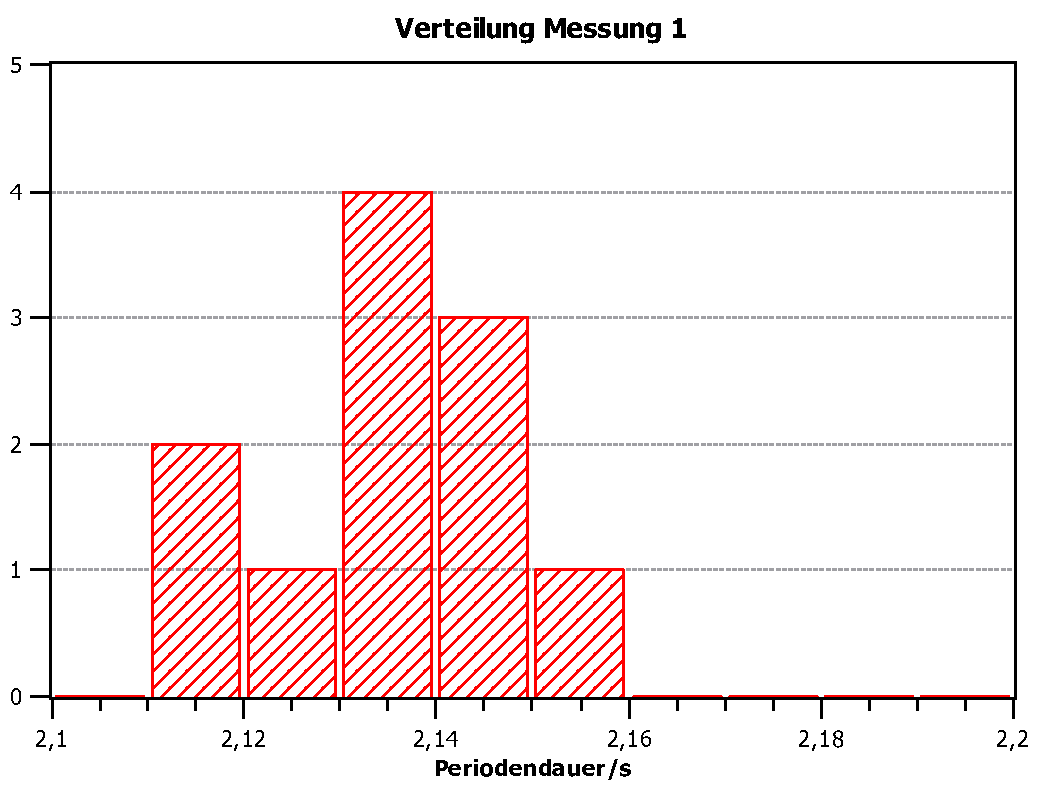
\includegraphics[width=\textwidth]{VerteilungMessung1.pdf}
			\caption{Messung für $L_1 = \SI{111,6}{\centi\meter}$}
			\label{fig:Hist1}
		\end{figure}
		\begin{figure}[ht]
			\centering
			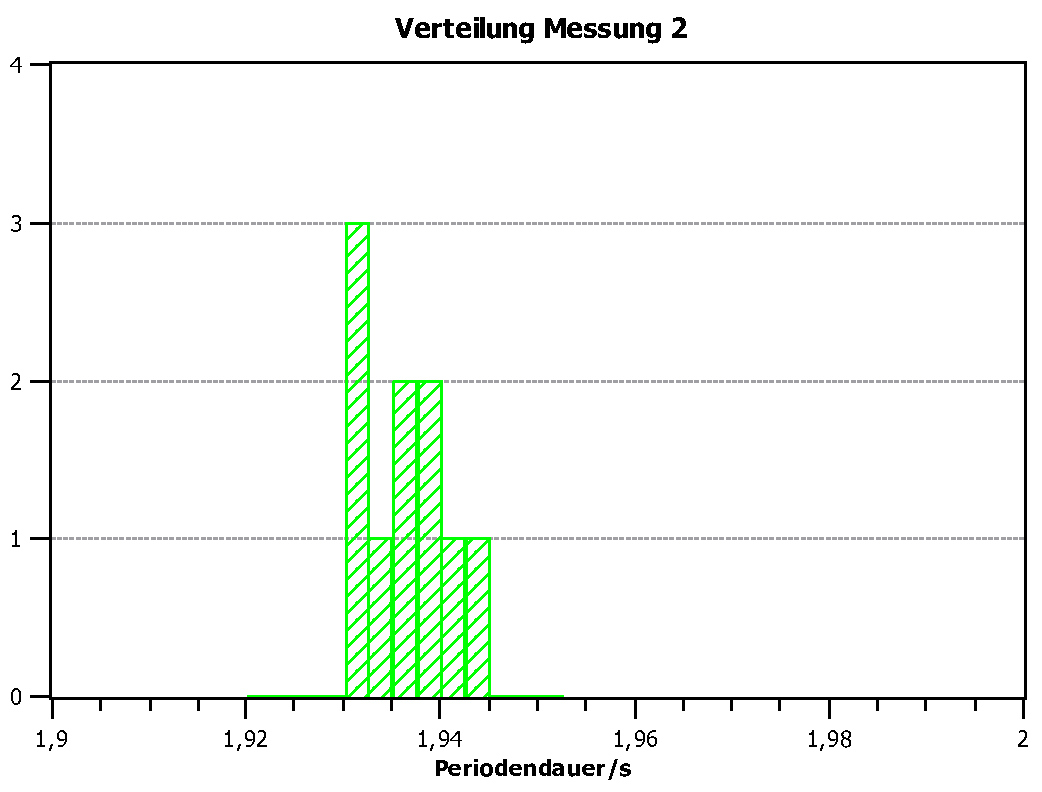
\includegraphics[width=\textwidth]{VerteilungMessung2.pdf}
			\caption{Messung mit $L_6 = \SI{92,6}{\centi\meter}$}
			\label{fig:Hist2}
		\end{figure}
			
		Die Abb. \ref{fig:multi} stellt die linearisierte Funktion $T^2 = \frac{4 \pi^2}{g} L$ (Gl. (\ref{eq:g}) nach $T^2$ umgestellt) dar.
		Die Unsicherheit $T^2$ muss nun neu berechnet werden mit $u(T^2) = \frac{\partial T^2}{\partial T} u(T) = 2 T \cdot u(T)$.
		Für die Seillänge können direkt die Werte aus (\ref{Messung} Messung) genommen werden.
		Bei der Funktion $T^2$ lässt sich ein Steigung von $m = \frac{4 \pi^2}{g}$.
		Mit der Ausgleichsgerade aus Abb. \ref{fig:multi} ist die Steigung $m = \SI{4,094}{\second\squared\per\meter}$.
		Die Unsicherheit muss mit Hilfe der Student'schen t-Verteilung korrigiert werden und beläuft sich bei $p = \SI{68,27}{\%}$ auf $u(m) = t_3 \cdot \SI{0,040}{\second\squared\per\meter} = \SI{0,047}{\second\squared\per\meter}$.
		
		\begin{figure}[ht]
			\centering
			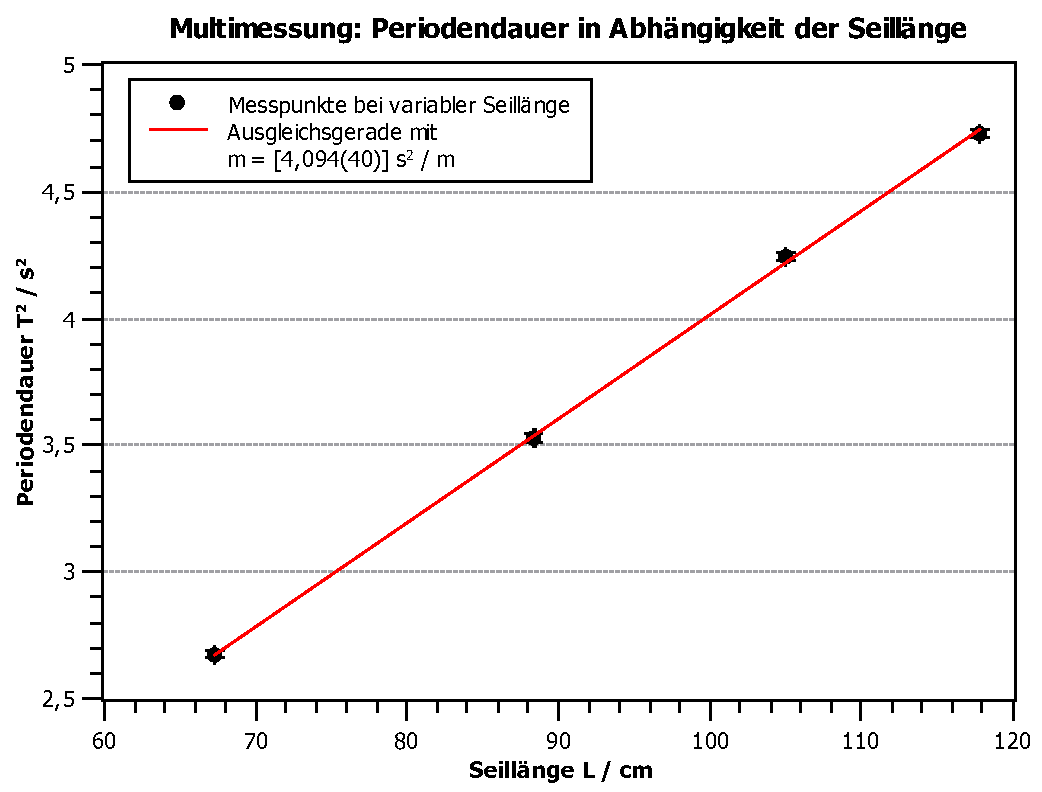
\includegraphics[width=\textwidth]{SteigungMultimessung_2.pdf}
			\caption{Datenpunkte der Multimessung mit Ausgleichsgerade. Die Unsicherheiten sind kleiner als die Symbole.}
			\label{fig:multi}
		\end{figure}
		
		Die kombinierte Unsicherheit $u(g)$ wird beschrieben durch
		\begin{equation*}
			m = \frac{4 \pi^2}{g} \Rightarrow g = \frac{4 \pi^2}{m};\quad 
			u(g) = -4\pi^2 \frac{u(m)}{m^2} \Rightarrow u(g) \approx \SI{0,1114}{\meter\per\second\squared}.
		\end{equation*}
		Dabei ist der Betrag der Unsicherheit wichtig.\\
		Damit folgt eine Gravitationskonstante von $g = \SI{9,643 +- 0,111}{\meter\per\second\squared}$.
		
	\section{Zusammenfassung}
		Durch ein Pendelexperiment haben wir die Gravitationskonstante auf einen Wert nahe dem Literaturwert ermittelt.
		Als mathematische Grundlage diente hierzu das ideale Pendel, wobei z. B. der Luftwiderstand ignoriert wurde.
		Zur weiteren Überprüfung haben wir mit zwei unterschiedlichen Messverfahren gearbeitet.
		Zum einen war die Seillänge des Pendels für eine große Anzahl an Messungen unverändert, zum anderen wurden mehrere kleinere Messreihen zu unterschiedlichen Seillängen durchgeführt und in Relation zur Periodendauer gesetzt.
		Dabei sind die Unsicherheiten für die Zeit- und Längenmessung berücksichtigt worden.
		
	\section{Schlussfolgerung}
		Nach eingehenden Untersuchungen zur Gravitationskonstante durch ein Pendel können wir die von der WWU gemessenen Größen nicht bestätigen.
		Unsere Ergebnisse deuten nämlich eindeutig darauf hin, dass die Gravitationskonstante nicht im Bereich von \SIrange{10,5}{11}{\meter\per\second\squared} liegt.
		Alle Messwerte liegen näher dem Literaturwert und erst bei großen Vertrauensgraden kann der WWU-Wert in Betracht gezogen werden.
		Die Gravitationskonstante in Münster unterliegt demnach keiner Anomalie und einem dem Literaturwert entgegengesetzten Wertes können wir mit unseren Ergebnissen nicht zustimmen.
		Es stellt sich die Frage, welche Faktoren Einfluss auf die Lichtschrankenmessung hatten, so dass sich Werte von $g$ ergaben, die so stark vom Literaturwert abweichen.
		Um das Problem der WWU-Messung zu finden, müsste man Nebeneffekte, wie z. B. die Luftreibung, genauer betrachten und diese berücksichtigen.
		
		\newpage
		
		\begin{thebibliography}{9}		
			\item[Abbildung 2:] \url{http://people.physik.hu-berlin.de/~mitdank/dist/scriptenm/pendel-Dateien/image001.gif}			
		\end{thebibliography}	
			
\end{document} 